\section{Retrieval}
\lable{sec:retrieval}

% \begin{itemize}
%     \item Query Processing
%     \item Hardware Support
%     \item Probabilistic output
%     \item online vs offline preprocessing
% \end{itemize}

With a trained model in hand, we are able to find documents in databases that the classifier has not seen before. However, classification and processing of every file in a database is resource and time intensive. Thus we use a combination of techniques to ensure that the right files are given by the database and it is accomplished quickly.

\subsection{Query Processing}
Previous attempts with audio retrieval have trained models not only on the audio itself but also the keywords associated with them. This simplifies the task of query processing, however this adds another layer of error that can propagate to the final results. Instead, in this preliminary system, the focus is on pure retrieval of documents based on audio content with the natural language processing problem of transforming queries into canonical forms is left for future work. However, simple transformations do take place.

\subsection{Ingest Cost vs Query Latency}
Most of the preprocessing steps are performed on the CPU and are not optimized for highly parallel architectures. Thus, the load times for a five second audio clip is approximately 250ms which means at scale with variable length audio and thousands, if not millions of records, this approach is infeasible for use at query time. However, front-loading too much of the work would result in a much larger ingestion cost, and as such a balance is pursued.
\\
\textbf{Processing at Ingestion Time.} \sys attempts to mitigate the computationally expensive task of processing the audio documents by transforming them to a feature vector that is saved in a table as the audio documents are added to the database. This increases the initialization cost of the system, with a database of approximately 2000 needing about 8 minutes and a database of 9500 needing about 50 minutes.

\begin{figure}[h]
    \centering
    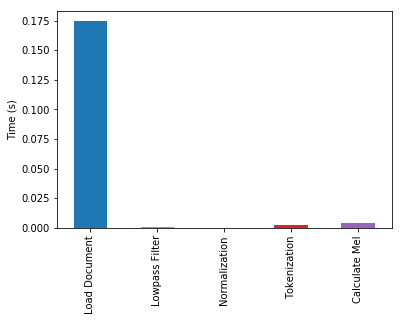
\includegraphics[width=.45\textwidth]{figures/Preprocessing-Timing-Factors.png}
    \caption{Time component of the preprocessing steps}
    \label{fig:time-component}
\end{figure}
